\documentclass[12pt]{article}
\usepackage[top=2cm,bottom=2cm,right=2.5cm,left=2.5cm]{geometry}
\usepackage[francais]{babel}
\usepackage[utf8]{inputenc}
\usepackage[T1]{fontenc}
\usepackage[absolute]{textpos} 
\usepackage{graphicx}
\usepackage{caption}
\usepackage{amsthm}
\usepackage{xcolor}
\usepackage[dvips,colorlinks=true,linkcolor=blue,urlcolor=blue,bookmarks=false,pdfpagemode=None]{hyperref}
\usepackage{listings}


\title{Raja \\ Bases de données distribuées \\ A Lire - Tutoriel}

\vspace{10mm}
\def\blurb{%
   Université des Sciences de Montpellier \\
  Master 2 Semestre 1 \\
  Unité d'Enseignement FMIN306
	}
\def\clap#1{\hbox to 0pt{\hss #1\hss}}%
\def\ligne#1{%
  \hbox to \hsize{%
    \vbox{\centering #1}}}%
\def\haut#1#2#3{%
  \hbox to \hsize{%
    \rlap{\vtop{\raggedright #1}}%
    \hss
    \clap{\vtop{\centering #2}}%
    \hss
    \llap{\vtop{\raggedleft #3}}}}%
\def\bas#1#2#3{%
  \hbox to \hsize{%
    \rlap{\vbox{\raggedright #1}}%
    \hss
    \clap{\vbox{\centering #2}}%
    \hss
    \llap{\vbox{\raggedleft #3}}}}%
\begin{document}
\thispagestyle{empty}\vbox to 1\vsize{%
  \vss
  \vbox to 1\vsize{%
    \haut{}{\blurb}{}
    \vfill
    \ligne{\Large \maketitle{}}
   % \vspace{5mm}
    \ligne{}
    \vfill
    \ligne{%
     }
    \vspace{15mm}
    \ligne{%
      \begin{tabular}{l}
	   Audrey \textsc{Novak}\\
        Romain \textsc{Maneschi}\\
	   Jonathan \textsc{Fhal}\\
	   Aloys \textsc{Urbain}
      \end{tabular}
      }
    }%
  \vss
  }

\newpage

\tableofcontents

\newpage

\section{Introduction}
	Dans ce tutoriel, nous vous présenterons comment installer notre application et comment l'utiliser pour notamment réaliser une requête de type \textit{Select}, \textit{Insert} ou \textit{Delete}. Mais également comment remplir le fichier de configuration pour pouvoir se connecter aux bases de données.
	Pour réaliser à bien ce tutoriel, nous partons du principe que le modèle ontologique à déjà été pré-fait, et que les fichiers owl des schémas locaux et du schéma global ont déjà été générés. De plus, n'ayant pas réussi à installer sur notre machine virtuelle le SGBD \texttt{PostGreSql}, nous ne ferons aucun exemple sur cela. \\
	\indent On part également du principe que nous sommes en distribué et donc que vous allez installer vos bases sur différents ordinateurs.
	
\section{Installation}
	Afin de trouver les sources de notre projet, il suffit de se rendre sur notre \href{https://code.google.com/p/raja/source/checkout}{google code}. Et de télécharger les sources du projet, ou de cliquer directement sur ce lien : \href{http://raja.lydiman.net/raja.tar.gz}{Sources}.\\
	\subsection{Importation des sources dans \texttt{Eclipse}}
	\indent Ensuite, il suffit d'ouvrir \texttt{Eclipse} et d'importer le projet, pour cela il faut faire : \textbf{File > New Project > Java Project}, une fenêtre s'ouvre alors, dans laquelle il faut selectionner dans la partie \textbf{Contents} (voir image ci-dessous) le dossier dans lequel sont situées nos sources, c'est à dire dans le dossier \textit{RAJA} de nos sources. 
	\begin{center}
	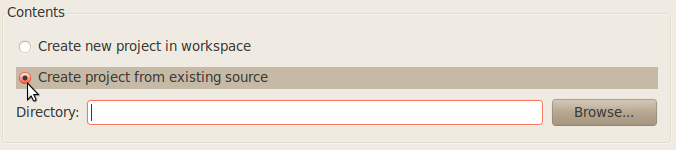
\includegraphics[scale=0.5]{Image/choisirProjet.png}
	\captionof{figure}{Importer les sources du projet}
\end{center}

	Il faut alors appuyer sur le bouton \textbf{Finish} pour terminer l'importation du projet dans le workspace d'\texttt{Eclipse}. \\
	
	\subsection{Installation des bases de données}
	Parmi le dossier des sources que vous avez téléchargé, vous trouverez dans le dossier \textit{BD} les différents scripts d'installation de nos bases. 
	\subsubsection{Base \texttt{Mysql}}
	On suppose que vous avez déjà installé le SGBD \texttt{Mysql}. Ouvrez un terminal situé dans le dossier \textit{BD} (pour pouvoir installer les tables sans inscrire le chemin absolu des scripts). Pour cela, tapez les commandes entourées en rouge dans l'image suivante : 
	\begin{center}
	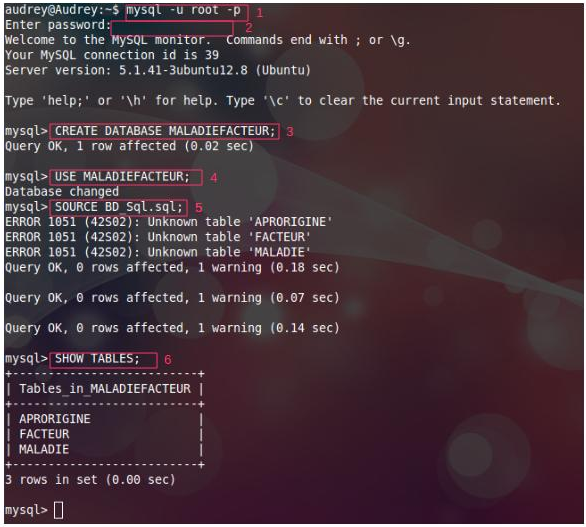
\includegraphics[width=0.8\textwidth]{Image/TerminalMysql.png}
	\captionof{figure}{Installer les bases \texttt{Mysql}}
\end{center}
	\textbf{Explications : }
	\begin{description}
		\item [1] Connection au SGBD \texttt{Mysql}
		\item [2] Entrez votre mot de passe utilisateur
		\item [3] Création de la base de données \textit{MALADIEFACTEUR}
		\item [4] Commande permettant de se placer et d'utiliser la base ainsi créée
		\item [5] Installation des tables à partir du script : \textit{BD\_Sql.sql}, les erreurs indiquées sont dues au fait que dans le script d'installation les premières lignes servent à effacer les tables, hors, comme nous sommes en train de les installer, elles n'existent pas encore, le système ne peux donc pas les trouver.
		\item [6] Commande permettant de voir quels sont les tables installées
	\end{description}
  	\indent Si vos manipulations ont réussi, vous devez obtenir la même image que nous. \\
  	\indent Il faut maintenant installer les tuples dans la base de données, pour cela, il faut entrer la commande suivante : \texttt{mysql > SOURCE Tuples\_Sql.sql}
	
	\subsubsection{Base \texttt{Oracle}}
	Il faut réaliser les mêmes actions que pour \texttt{Mysql}, on part également du principe que \texttt{Oracle} est déjà installé sur votre ordinateur, et qu'il est correctement configuré (notamment pour les utilisateurs et pour la base principale d'oracle).
	\begin{center}
	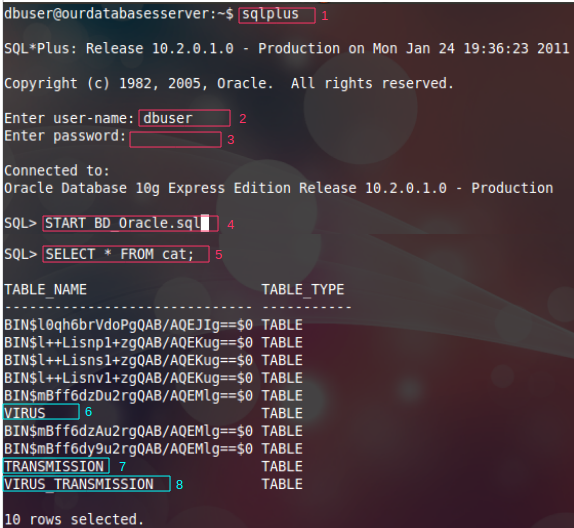
\includegraphics[width=0.80\textwidth]{Image/TerminalOracle.png}
	\captionof{figure}{Installer les bases \texttt{Oracle}}
\end{center}
		\textbf{Explications : }
	\begin{description}
		\item [1] Connection au SGBD \texttt{Oracle}
		\item [2] Entrez votre nom d'utilisateur
		\item [3] Entrez votre mot de passe
		\item [4] Commande permettant d'installer les tables à partir du script : \textit{BD\_Oracle.sql}. L'image que nous vous présentons est un montage, nous avons coupé la partie d'installation des tables pour réduire l'image.
		\item [5] Commande permettant d'afficher toutes les tables installée dans la base de données.
		\item [6-7-8] Résultat que l'on obtient après la commande \textbf{5}, on voit bien que les tables \textit{VIRUS, TRANSMISSION et VIRUS\_TRANSMISSION} ont bien été installées.
	\end{description}
	\indent En suivant correctement ce tutoriel, vous devriez donc obtenir ce résultat. \\
	\indent Il faut également installer les tuples dans nos tables, pour cela tapez : \texttt{sql > START Tuples\_Oracle.sql}
	\\
	\\
	\indent Pour installer les bases de recensements qui sont découpées horizontalement par zones, il suffit de réaliser la même méthode, une fois pour la base recensementEurope et une fois pour la base recensementEastEurope. \\
	\\
	\indent Le projet est alors installé, il faut maintenant remplir le fichier de configuration pour pouvoir se connecter aux bases de données.
	
\section{Configuration}
	\subsection{Fichier de configuration}
	Le fichier de configuration de notre système est un fichier xml. Pour le créer vous pouvez vous inspirez du fichier \textit{RAJA/ConfigOriginal/config.xml} ouvert avec un éditeur de texte, on voit alors que ce fichier est composé de divers noeuds : un noeud pour chaque \textit{compositeAdaptater}, contenant le chemin vers le fichier owl concerné par ce \textit{compositeAdaptater}, la liste des préfixes relatifs à ce \textit{compositeAdaptater}, un noeud pour le \textit{terminalAdaptater} contenant l'adresse du fichier n3 à charger, et les méthodes de connection à la base de données, et ce pour chaque base de données. Vous pouvez ainsi ajouter autant de composites que nécessaire afin de structurer toutes vos données. Par la suite il vous suffit de remplacer la ligne 27 du fichier \textit{MyTabbedPane.java} pour la partie graphique et/ou la ligne 245 du fichier \textit{Server.java} pour le server en console. Enfin vous pouvez également remplacer \textit{new InddorFile()} de la ligne 245 du \textit{Server.java} par \textit{new IndoorConsole()} afin que le serveur vous demande une requête par la console plutôt que par un fichier. De même vous pouvez modifier l'url des fichiers pour le \textit{IndoorFile}. Enfin si vous utilisez un \textit{IndoorFile} vous pouvez commenter certaines lignes (pour ne pas les exécuter à chaque fois, ou pour des remarques par exemples) en la commençant par un dièse.\\
	\indent Ci-dessous nous vous présentons une version simplifiée de notre fichier de configuration, les éléments entourés sont les éléments qu'il faut modifier.
	\begin{center}
	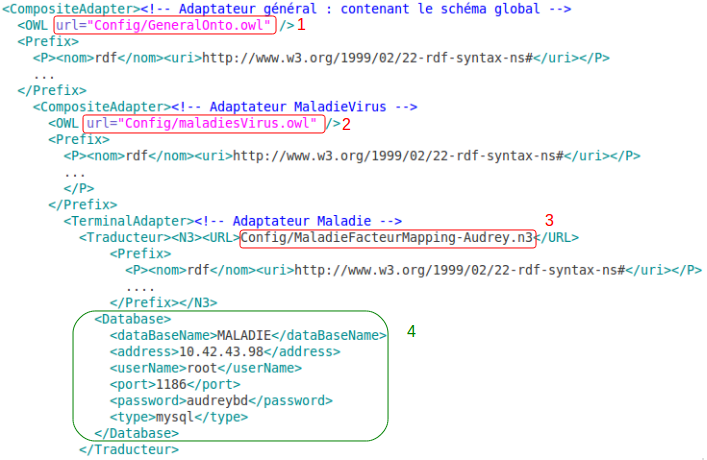
\includegraphics[width=0.90\textwidth]{Image/config.png}
	\captionof{figure}{Fichier de configuration}
\end{center}
	Pour chaque noeud \textit{CompositeAdaptater}, il faut réaliser les manipulations suivantes :
	\begin{description}
	\item [1-2] Indiquer l'adresse du fichier owl du modèle ontologique global (1), et du modèle ontologique local(2), ici de la base \textit{MALADIEFACTEUR}
	\item [3] Indiquer le chemin vers le fichier N3
	\item [4] Cet espace représente toute la configuration que vous devez effectuer pour configurer l'accès à la base de données. 
	\end{description}
	\indent Il ne faut pas changer les parties concernant les préfixes.
	
	\subsection{Fichier N3}
	Les fichiers N3 représentent la transformation de nos tables en classes et de leurs champs en propriétés de classes, ces fichiers ont également besoin d'être configurer pour que l'accès à la base de données se fasse sans problème.\\
	\indent Ci-dessous, vous trouverez un exemple d'entête de fichier N3 permettant l'accès à la base de données : 
	\begin{center}
	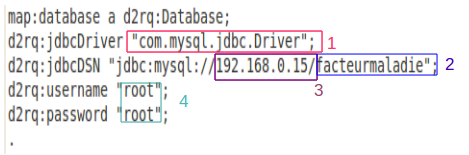
\includegraphics[width=0.70\textwidth]{Image/configN3.png}
	\captionof{figure}{Entête de fichier N3, configuration}
\end{center}
	\indent Cet exemple montre la configuration dans un fichier N3, pour une connection à une base de données sous \texttt{Mysql}. \\
	\indent Voici ce qu'il vous faut remplacer, en fonction de vos informations de connection : 
	\begin{description}
		\item [1] Indiquer le driver de votre base de données, dans le cas où votre base de données est sous \texttt{Mysql}, laissez celui-ci, si elle est en \texttt{Oracle}, remplacez cette partie par : \\ \texttt{oracle.jdbc.driver.OracleDriver}
		\item [2-3] Cette partie concerne la localisation de la base, plus particulièrement :  \textbf{2} = Nom de la base de données concernée par ce fichier \textbf{3} = Adresse de l'hôte sur lequel se trouve cette base. Plus généralement, pour \texttt{Mysql} voici ce que vous devez mettre : \\ \texttt{jdbc:mysql://NomHote:port/NomBase} ;\\ pour une base sous \texttt{Oracle} vous devez inscrire : \\ \texttt{jdbc:oracle:thin:@NomHote:Port:NomBase}, \\ le NomHote peut être remplacé par l'adresse IP de l'hôte.
		\item [4] Cette partie concerne plus particulièrement vos identifiants et mots de passe pour permettre l'autorisation de l'accès à la base de données.		
	\end {description}
	
	\\
	\\
	\indent A cette étape, votre application est configurée, vous pouvez dès lors la lancer.
\newpage
\section {Prise en main de notre application}
	\subsection{Application console}
	Pour lancer l'application console, rendez-vous dans \texttt{Eclipse}, dans le dossier \textit{src/Server/Server.java}, puis clic droit \textbf{Run As > Java Application}. \\
	Nous avons utilisé un fichier de test qui s'exécute lors du lancement de l'application console, vous devez normalement voir le résultat d'une requête dans la console. Le fichier test sera expliqué dans la partie suivante.
	Dans ce tutoriel, nous concentrerons notre explication sur l'application graphique de notre projet.
	\subsection{Application graphique}
	Pour lancer l'application graphique, il faut dans \texttt{Eclipse}, lancer de la même façon que pour l'application console, le fichier suivant : \textit{src/Server/Indoor/Graphic/MainWindow.java}. \\
	\indent La fênetre suivante s'ouvre alors : 
	\begin{center}
	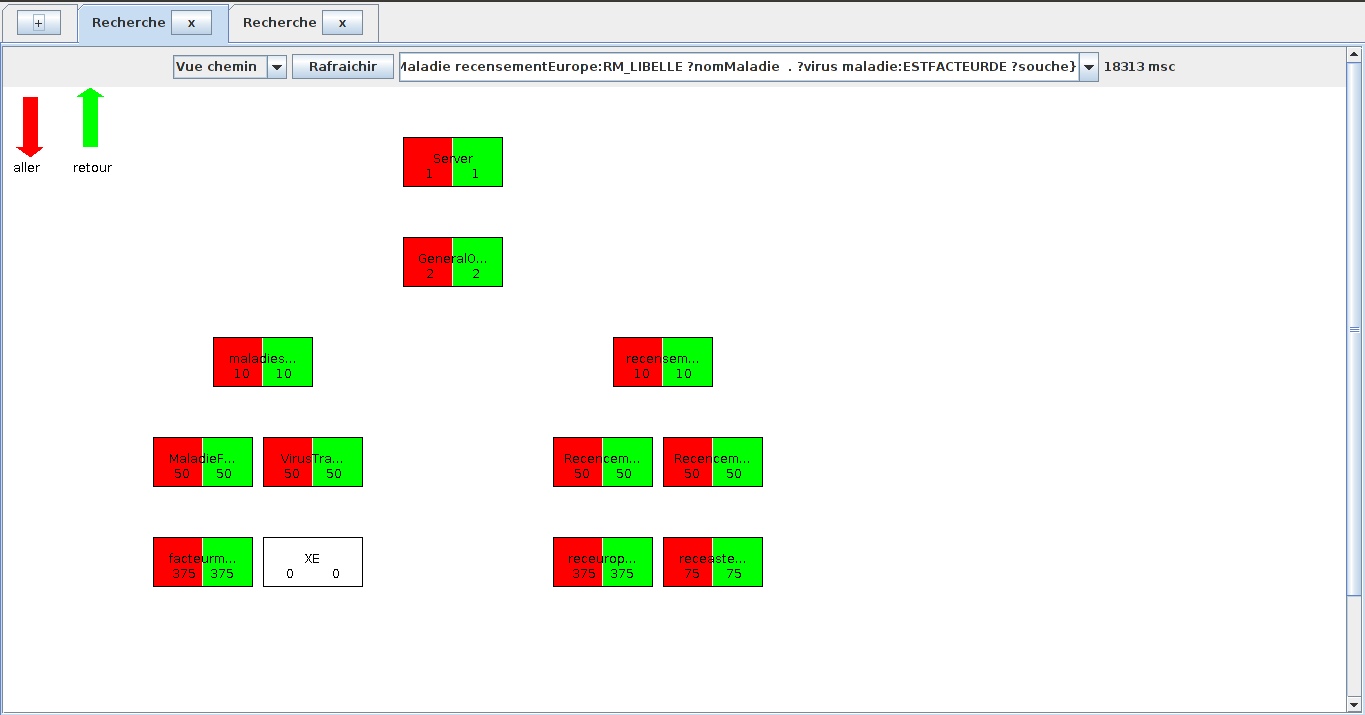
\includegraphics[width=1\textwidth]{Image/appli.png}
	\captionof{figure}{Application}
	\begin{itemize}
	\item L'application est composée d'une comboBox dans laquelle vous pouvez entrer vos requêtes sous forme de requêtes \texttt{SPARQL} pour les requêtes de type select ou en \texttt{SQL} pour les requêtes d'insertion et de supression. \\
	\indent De plus, comme vous pouvez le voir, la comboBox est pré-remplie, en effet, nous avons réalisé un test contenant plusieurs requêtes pré-faites, pour visionner ce fichier allez dans : \textit{src/Test.txt}. Ce fichier contient pour chaque requête, une explication en langage naturel de la requête.
	\item L'application est composée d'onglets, vous pouvez ainsi faire une requête par onglet.
	\item Une seconde comboBox est présente, elle permet de visionner le résultat de la requête de deux façons différentes : sous forme de triplets rdf, en cliquant sur : \textbf{Vue Modèle}, mais aussi sous forme de tableau en cliquant sur : \textbf{Vue Tableau}.
	\item Il est également possible de voir que la requête effectuée est allée dans la bonne base de données en cliquant sur \textbf{Vue Chemin}.
	\end{itemize}
\end{center}
\section{Faire une requête de sélection}
	La requête de sélection doit être faite en \texttt{SPARQL}, nous estimons ici que vous connaissez le système de requêtes de \texttt{SPARQL}. \\
	\indent Pour avoir une connaissance des différents liens qu'il existe entre nos tables, nous vous conseillons de réaliser la requête permettant d'obtenir le schéma global de notre système dans un premier onglet : \texttt{SELECT ?a ?b ?c WHERE \{?a ?b ?c\} } \\
	\indent Ouvrez maintenant un nouvel onglet, et servez vous du schéma global pour réaliser vos requêtes de sélection.
	
\section{Insérer une ligne}
	L'insertion de ligne est réalisé en SQL, nous estimons également qu'avant de réaliser ce tutoriel, vous avez des connaissances en SQL. Une requête d'insertion aura la forme : 
	\begin{itemize}
	\item La base recensement est divisée horizontalement par zone oms, donc pour réaliser l'insertion, dans ces tables, il est indispensable de préciser le nom de la base de données (\textit{receurope} ou \textit{receasteurope}), ainsi que le nom de la table dans laquelle on veut insérer, la requête est alors de la forme : \texttt{INSERT INTO nomBase.NomTable VALUES(v1,...,vn)}
	\item Pour les autres bases, qui sont découpées verticalement, il suffit juste d'indiquer le nom de la table dans laquelle on veut insérer, la requête est donc de la forme : \texttt{INSERT INTO nomTable VALUES(v1,...,v2)}
	\end{itemize}
		
\section{Supprimer une ligne}
	Pour supprimer une ligne, vous devez également faire votre requête en \texttt{SQL}. 
		\begin{itemize}
	\item Suppression d'une ligne dans la base recensement : en raison du découpage horizontal, il faut comme pour la requête d'insertion, indiquer la base dans laquelle on veut supprimer la ligne et le nom de la table concernée, voici la forme de la requête que vous devez faire : \texttt{DELETE FROM nomBase.nomTable WHERE condition;}
	\item Pour les autres bases, qui sont découpées verticalement, il suffit juste d'indiquer le nom de la table dans laquelle on veut supprimer la ligne, la requête est donc de la forme : \texttt{DELETE FROM nomTable WHERE condition;}
	\end{itemize}
	
\section{Conclusion}
	Nous espérons que ce tutoriel vous aura été utile pour prendre en main notre application, nous vous prions de faire remonter les bugs que vous auriez trouvé sur la page : \href{https://code.google.com/p/raja/issues/list}{Issues de Google code}.
\end{document}
